%!TeX program=pdflatex
%!TeX encoding=utf8
%!TeX spellcheck = en_US
%!TeX root = ../../messageVortex.tex

\partepigraph{No matter how hard you work, someone else is working harder.}{Elon Musk, entrepreneur}
\part{Implementation\label{sec:implementation}}
The implementation differs from the academic model in some details. It is formeost more precise than the academic model. Furthermore it requires a strict definition of the implementation in order to guarantee the interoperability between different implementations.

This section focusses therefore on the implementation details of the reference implementation.

\chapter{Selection of Algorithms and Protocols}
\section{Algrorithm Selection}
\subsection{Cryptographic Algorithms}
\subsubsection{Cipher Selection}
In this protocol, a lot of encryption and hashing algorithms have to be used. This choice of these algorithms should be explained. 

From the requirements side, we have to follow the following principle:
First of all, we need a subset of encryption algorithms all implementations may rely on. Defining such a subset guarantees interoperability between all nodes regardless of their origins. 

Secondly, we need to have a spectrum of algorithms in such a manner that it may be (a) enlarged if necessary and (b) there is an alternative if an algorithm (or a mathematical problem class) is broken (so that algorithms may be withdrawn if required without affecting the function in general). 

And third, due to the onion-like design described in this document, asymmetric encryption should be avoided in favor of symmetric encryption to minimize losses due to the key length and the generally higher CPU load opposed by asymmetric keys.

If the algorithm is generally bound to specific key sizes (due to S-Boxes or similar constructs), the key size is incorporated into the definition. If not, the key size is handled as a parameter.

The key sizes have been chosen in such a manner that the key types form tuples of approximately equal strength. The support of Camelia192 and Aes192 has been defined as optional. However, as they are wildly common in implementations, they have already been standardized as they build a possibility to step up security in the future.

Having these criteria for choice, we chose to use the following keys and key sizes:
\begin{itemize}
	\item Symmetric
	\begin{itemize}
		\item AES (key sizes: 128, 192, 256)
		\item Camellia (key sizes: 128, 192, and 256)
	\end{itemize}
	\item Asymmetric
	\begin{itemize}
		\item RSA (key size: 2048, 4096, and 8192)
		\item Named Elliptic Curves
		\begin{itemize}
			\item secp384r1
			\item sect409k1
			\item secp521r1
		\end{itemize}
	\end{itemize}
	\item Hashing
	\begin{itemize}
		\item sha3-256
		\item sha3-384
		\item sha3-512
		\item RIPE-MD160
		\item RIPE-MD256
		\item RIPE-MD320
	\end{itemize}
\end{itemize}

Within the implementation, we assigned algorithms to a security strength level:
\begin{itemize}
	\item LOW\\
	AES128, Camellia128, RSA1024, sha3-256
	\item MEDIUM\\
	AES192, Camellia 192, RSA2048, ECC secp384r1, sha3-256
	\item HIGH\\
	AES256, Camellia256, RSA4096, ECC sect409k1, sha3-384
	\item QUANTUM\\
	AES256, Camellia256, RSA8192, ECC secp521r1, ntru, sha3-512
\end{itemize}

This allows categorizing the used algorithms to a strength. This list, however, should only serve the purpose of selecting algorithms for people without cryptological know-how.

\subsubsection{Mode Selections}
We evaluated the most common cipher modes for suitability. For MessageVortex, we focussed on modes that have the properties parallelizable, random access, and do not do authentication. The main focus, besides the characteristics mentioned before, was on the question of whether there is an open implementation available in java, which is reasonably tested.

\begin{itemize}
	\item ECB (Electronic Code Book)\\
	      ECB is the most basic mode. Each block of the cleartext is encrypted on its own. This results in a big flaw: blocks containing the same data will always transform to the same ciphertext. This property makes it possible to see some structures of the plain text when looking at the ciphertext. This solution allows the parallelization of encryption, decryption, and random access while decrypting. Due to these flaws, we rejected this mode.
	\item CBC (Cypher Block Chaining)\\  
	      CBC extends the encryption by xor'ing an initialization vector into the first block before encrypting. For all subsequent blocks, the ciphertext result of the preceding block is taken as xor input. This solution does not allow parallelization of encryption, but decryption may be paralleled, and random access is possible. As another downside, CBC requires a shared initialization vector. As with most IV bound modes, an IV/key pair should not be used twice, which has implications for our protocol.
	\item PCBC (Propagation Cypher Block Chaining)\\
	      CBC extends the encryption by xor'ing, not the ciphertext but a xor result of ciphertext and plaintext. This modification denies parallel decryption and random access compared to CBC.
	\item EAX\\      
	      EAX has been broken in 2012\cite{minematsu2013attacks} and is therefore rejected for our use.
	\item CFB (Cypher Feedback)
	      CFB is specified in \cite{dworkin2001recommendation} and works precisely as CBC with the difference that the plain text is xor'ed and the initialization vector, or the preceding cipher result is encrypted. CFB does not support parallel encryption as the ciphertext input from the preceding operation is required for an encryption round. CFB does, however, allow parallel decryption and random access.
	\item OFB\\
	      \cite{dworkin2001recommendation} specifies OFB and works exactly as CFB except for the fact that not the ciphertext result is taken as feedback but the result of the encryption before xor'ing the plain text. This denies parallel encryption and decryption, as well as random access.
	\item OCB (Offset Codebook Mode)\\
	      This mode was first proposed in \cite{rogaway2003ocb} and later specified in \cite{krovetz-ocb-04}. OCB is specifically designed for AES128, AES192, and AES256. It supports authentication tag lengths of 128, 96, or 64 bits for each specified encryption algorithm. OCB hashes the plaintext of a message with a specialized function $H_{OCB}(\mathbf{M})$. OCB is fully parallelizable due to its internal structure. All blocks except the first and the last can be encrypted or decrypted in parallel.
	\item CTR\\
	      CTR is specified in \cite{lipmaa2000ctr} and is a mixture between OFB and CBC. A nonce concatenated with a counter incrementing on every block is encrypted and then xor'ed with the plain text. This mode allows parallel decryption and encryption, as well as random access. Reusing IV/Key-pairs using CTR is a problem as we might derive the xor'ed product of two messages. This problem only applies where messages are not uniformly random such as in an already encrypted block.
	\item CCM\\
	      Counter with CBC-MAC (CCM) is specified in \cite{RFC3610}. It allows to pad and authenticate encrypted and unencrypted data. It furthermore requires a nonce for its operation. The size of the nonce is dependent on the number of octets in the length field. In the first 16 bytes of the message, the nonce and the message size is stored. For the encryption itself, CTR is used. It shares the same properties as CTR. 
	
	      It allows parallel decryption and encryption as well as random access.
	\item GCM (Galois Counter Mode)\\
	      GCM has been defined in \cite{mcgrew2004galois}, and is related to CTR but has some major differences. The nonce is not used (just the counter starting with value 1). To authenticate the encryption, an authentication token $auth$ is hashed with $H_{GFmult}$ and then xor'ed with the first cipher block. All subsequent cipher blocks are xor'ed with the previous result and then hashed again with $H_{GFmult}$. After the last block the output $o$ is processed  as follows: $H_{GFmult}(o\bigoplus (len(A)||len(B))) \bigoplus E^{K^0}(counter_0)$. As a result, GCM is not parallelizable and does not support random access.
	
	      The mode has been analyzed security-wise in \citeyear{mcgrew2004security} and showed no weaknesses in the analyzed fields \cite{mcgrew2004security}. 
	
	      GCM supports parallel Encryption and decryption. Random access is possible. However, authentication of encryption is not parallelizable. The authentication makes it unsuitable for our purposes. Alternatively, we could use a fixed authentication string.
	\item XTS (XEX-based tweaked-codebook mode with ciphertext stealing)\\
	      This mode is standardized in IEEE 1619-2007 (soon to be superseded). A rough overview of XTS may be found at \cite{Martin2010}. It was developed initially for Disks offering random access and authentication at the same time. 
	\item CMC (CBC-mask-CBC) and EME (ECB-mask-ECB)\\ 
	      In \cite{Halevi:2003} \citeauthor{Halevi:2003} introduces a cipher mode which is extremely costly as it requires two encryptions. CMC is not parallelizable due to the underlying CBC mode, but EME is. 
	\item LRW\\
	      LRW is a tweakable narrow-block cipher mode described in \cite{tschorsch:translayeranon}. This mode shares the same properties as EBC but without the weakness of the same clear text block resulting in the same ciphertext. Similarly to XEX, it requires a tweak instead of an IV.
\end{itemize}



\subsubsection{Padding selection}
A plain text stream may have any length. Since we always encrypt in blocks of a fixed size, we need a mechanism to indicate how many bytes of the last encrypted block may be safely discarded. 

Different paddings are used at the end of a cipher stream to indicate how many bytes belong to the decrypted stream.

\subsubsection{RSAES-PKCS1-v1\_5 and RSAES-OAEP}
This padding is the older of the paddings standardized for PKCS1. It is basically a prefix of two bytes followed by a padding set of non zero bytes and then terminated by a zero byte and then followed by the message. This patting may give a clue if decryption was successful or not. RSAES-OAEP ist the newer of the two padding standards 

\subsubsection{PKCS7} 
This padding is the standard used in many places when applying symmetric encryption up to 256 bits key length. The free bytes in the last cipher block indicate the number of bytes being used. This makes this padding very compact. It requires only 1 Byte of functional data at the end of the block. All other bytes are defined but not needed.

\subsubsection{OAEP with SHA and MGF1 padding} 
This padding is closely related to RSAES-OAEP padding. The hash size is, however, bigger, and thus, the required space for padding is much higher. OAEP with SHA and MGF1 Padding is used in asymmetric encryption only. Due to its size, it is important to note that the payload in the last block shrinks to $keySizeInBits/8-2-MacSize/4$.

In our approach, we have chosen to allow these four paddings. The allowed sha sizes match the allowed mac sizes chosen above. It is important to note that padding costs space at the end of a stream. Since we are always using one block for signing, we have to take care that the chosen signing mac plus the bytes required for padding do not exceed the key size of the asymmetric encryption. While this usually is not a problem for RSA as there are keys 1024+ Bits required, it is an essential problem for ECC algorithms as there are much shorter keys needed to achieve an equivalent strength compared to RSA. 

We have introduced an additional type of padding not related to these paddings. We required for the addRedundancy the following unique properties. Unfortunately, we were unable to find any padding which matched the following properties simultaneously:

\begin{itemize}
	\item Padding must not leak successful decryption\\
	For our addRedundancy operation, we required padding that had no detectable structure as a node should not be able to tell whether a removeRedundancy operation did generate content or decoy. 
	\item Padding of more than one block\\
	Due to the nature of the operation, it is required to be able to pad more than just one block.
\end{itemize}

\subsection{Pseudo Random Number Generator Selection\label{sec:prng}}
For our $addRedundancy$ and $removeRedundancy$ operations we needed a pseudo random number generator (PRNG). For our implementation we did not research deeply this part as it seemed irrelevant. The only criteriion was, that it had to create content indistinguishable from an encrypted message. This criterion arose as we use it for padding invisibly an already encrypted message.

The PRNG used for our implementation is an xorshift+ generator. It is based on the XSadd PRNG\cite{marsaglia2003xorshift} and passes the bigcrush PRNG test suite. It is a fast, xor based PRNG which has two internal 64 bit seed states $s_0$ respectively $s_1$ and is defined as follows:

\begin{eqnarray}
x & = & s_0\\
s_0 & = & s_1\\
x & = & x \oplus ( x \ll 23 )\\
s_1 & = & x \oplus s_1 \oplus ( x \gg 17 ) \oplus (s_1 \gg 26 )\\
nextNumber & = & s_1+s_0
\end{eqnarray}

We have chosen this comparably weak PRNG for practical reasons. It is fast, simple, and is based on operations easy to implement on hardware. As we do not need a cryptographically strong PRNG, it is our primary choice so far. 

As the protocol is heavily dependent on security we have introduced everywhere at least one alternate algorithm which may be used if one of the choices may become a problem. In order to have a second choice for the PRNG we define the Blum-Micali PRNG as described in \cite{blum1984generate}. This PRNG is a cryptographically secure PRNG and is defined as follows:

$p$ is prime and $g$ is a primitive root modulo $p$. $x_0$ reflects the seed state.

\begin{eqnarray}
x_{i+1}=g^{x_i}\mod p
\end{eqnarray}

\subsection{Puzzle Selection}
\fxwarning{Add content here... maybe old text about PoW-Algorithms}

\section{Protocol Selection}
\subsection{Transport Layer Protocol Selection}
In order to be truly agnostic and inter-operable, we had to test our environment under multiple transport layers. At the same time we needed mechanisms allowing us to add protocol support at any level at a later stage.

While implementation of the standard protocols has proven to be straight forward we discovered \fxwarning{ FIX text and ToC here}

\chapter{Transport Layer Implementation}
\section{Implementation of a Dummy Transport Layer}

\section{Implementation of a Email Transport Layer}

\section{Implementation of an XMPP Transport Layer}

\chapter{Blending Layer Implementation}
\section{Embedding Spec}
We always embed VortexMessages as attachments in SMTP and XMPP messages. 

The embedding supports some properties. A receiving host chooses the supported properties. We describe valid properties by the blending specification::
\begin{lstlisting}[language=EBNF]
plainEncoding = "("plain:"<#BytesOfOffset>[,<#BytesOfOffset>]*")
F5Encoding    = "(F5:"<passwordString>[,<PasswordString>]*")"
\end{lstlisting}

\subsection{Plain Embedding}
The $plainEncoding$ is a simple embedding replacing the original file with the content of the \VortexMessage. To maintain the header information of a file we introduced an offset as a set of fixed values. A plain embedding may be identified by a host when decoding a single block with $K^{-1}_{host_o}$ if the resulting structure is an ASN.1 stucture is equivalent to XXX.


We use mainly plain embedding for our experiments. For better readability, we used a specialized blending layer using unchunked, plain embedding with an offset of $0$. The message itself was the ASN.1 block representation of the encoded block. The chosen encoding simplified to see the inner workings of the protocol. For production use, we apply F5 embedding with a generated payload. The current implementation of the blending layer employing plain embedding is thus not suitable for production use as the messages remain identifiable or at least suspicious.

\subsubsection{Chunking of Plain Embedded Messages}\label{sec:chunkingPlain}
\fxwarning{complete section}

\subsection{implementation of F5 Blending}
\fxwarning{complete section}

\chapter{Routing Layer Implementation}
\fxwarning{complete section}
\section{ASN.1 encoding scheme}
Originally, we implemented the protocol as XML encoded messages. This encoding had, however, several flaws. First the huge ammount of encrypted data within the document made the messages bulky and at the same time loose one of its main strengths: readability for humans. The encoding required for binary data caused messages to increase ion size due to their onionized structure. 

Furthermore, the complex XML features \fxwarning{incomplete section}

\section{Processing of messages}
\fxwarning{complete section}

\subsection{Processing of Incoming Messages}\label{sec:processingIncommingMessages}
A Block is picked up in the blending layer and then handled in the routing layer. First, we try to authenticate the message. If we can authenticate the message, we process it and add the contained instructions to a processing workspace. Unauthenticated messages may be discarded at any point.

The processing of a sending block is triggered by a routing block in the workspace, as shown in figure~\ref{fig:msgSendProcessing}. The assembly instructions are processed to collect the payload blocks. Then the encryption is applied to the message and passed on to the blending layer for processing.

\begin{figure*}[hbt]
	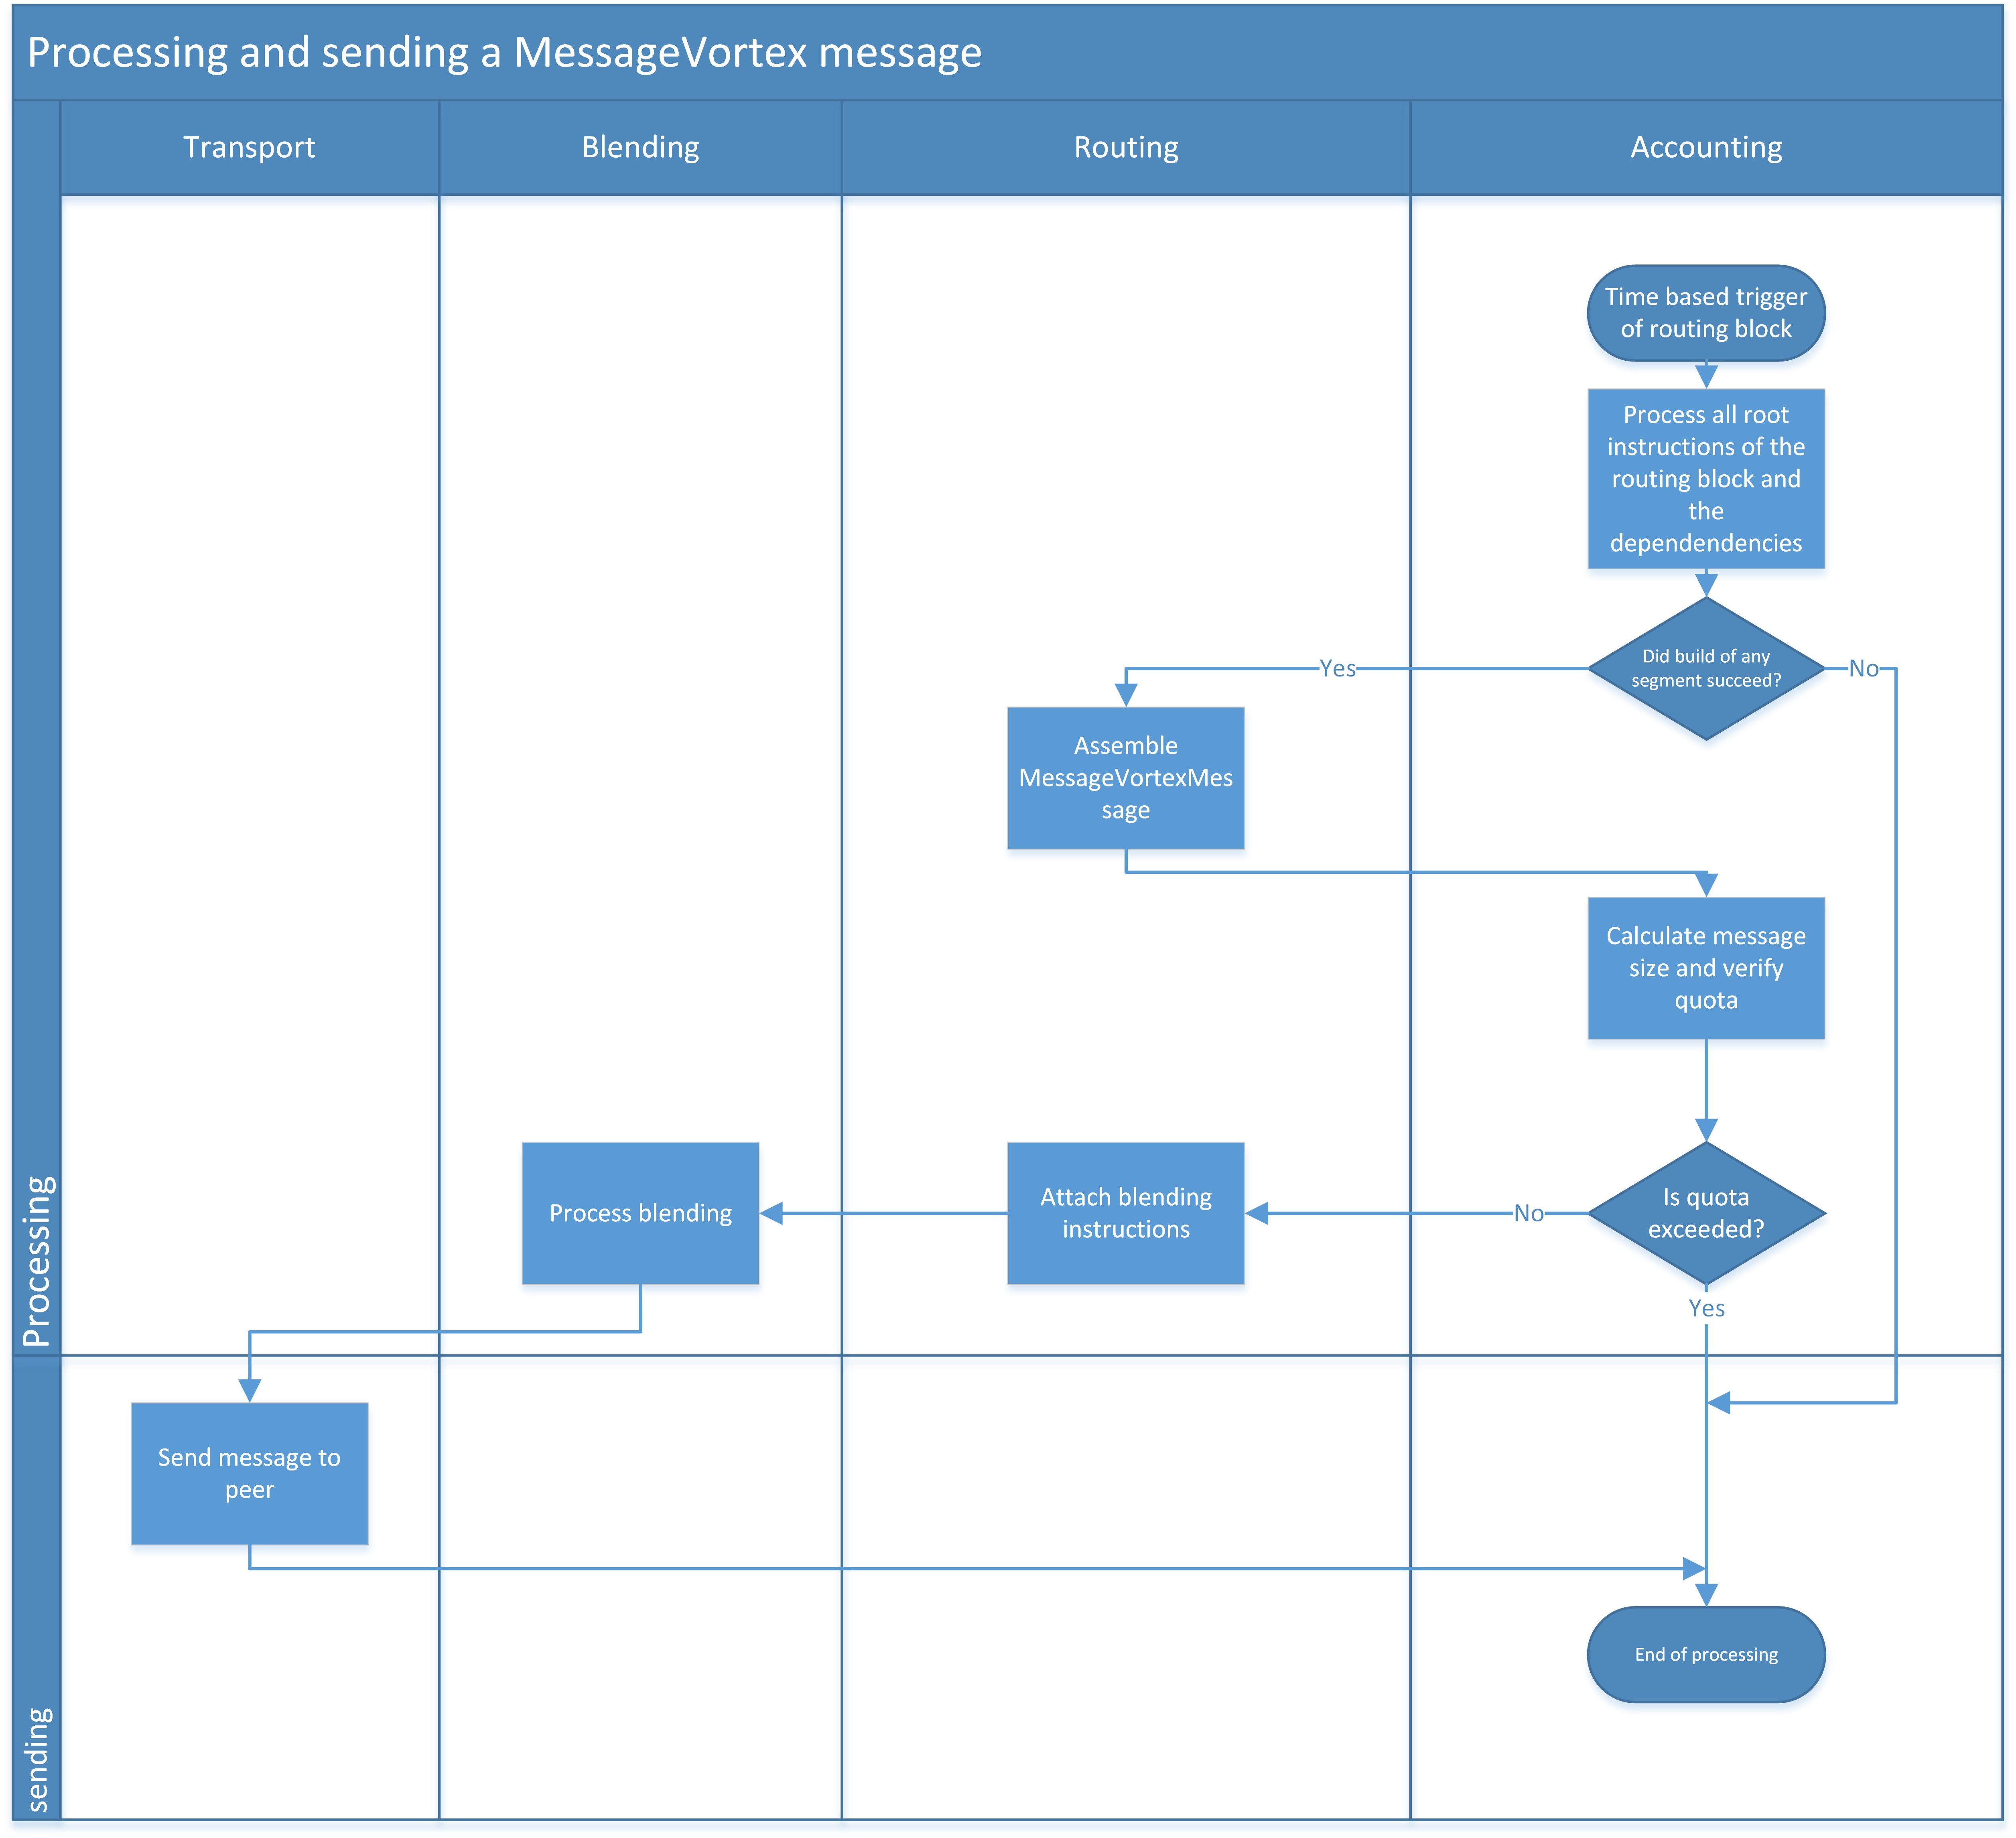
\includegraphics[width=0.90\textwidth]{inc/flowchart_message_sending}
	\caption{flow diagram showing processing of outgoing messages}
	\label{fig:msgSendProcessing}
\end{figure*}

\fxwarning{complete section}

\subsection{Processing of Outgoing Messages}\label{sec:processingOutgoingMessages}
\fxwarning{complete section}

\subsection{Implementation of Operations}\label{sec:implOperations}
\fxwarning{Mention mapping operation}

\fxwarning{Mention floating point issues when splitting}

\fxwarning{complete section}

\section{Request handling}
\fxwarning{complete section}

\subsection{Requesting a new Ephemeral Identity}\label{sec:newEID}
\fxwarning{complete section}

\subsection{Replacing an Existing Node Identity}
\fxwarning{complete section}

\subsection{Replacing an Existing Reply Block}\label{sec:replaceMURB}
\fxwarning{complete section}


\chapter{Accounting Layer Implementation}
\fxwarning{complete section}

\chapter{Usability Related Implementation Details}
\fxwarning{complete section}

\section{Adressing and address representations}
\fxwarning{complete section}

\section{Linking to Common User Agents}
\fxwarning{complete section}

\chapter{Efficiency Related Implementation Details}
\fxwarning{complete section}

\section{Node Storage Management}
\fxwarning{complete section}

\subsection{Life-cycle of Ephemeral Identities and Workspaces}
\fxwarning{complete section}

\subsection{Life-cycle of Requests}
\fxwarning{complete section}

\subsection{Life-cycle of Operations}
\fxwarning{complete section}

